\section{Experimental Setup}\label{sec:experimentalSetup}

The goal of this research is to build an in-depth understanding about
the performance of the \mas for detecting malware. To this
end, we conduct our research using a dataset one order of magnitude
larger than previous studies. We also investigate to what
extent variants of the \mas achieve a better performance
for malware detection. Altogether, our
aim is to answer the following research questions:

\begin{enumerate}[(RQ1)]
\item \rqa
\item \rqb
\item \rqc  
\end{enumerate}

In this section, we describe our study settings. First, we present how we mined the data-set of Android app pairs that we
use as a benchmark for our study (Section~\ref{sec:dataset}).  Then, we describe the data collection and
data analysis procedures in Sections~\ref{sec:dataCollectionProc} and~\ref{sec:dataAnalysisProc},
respectively. Section~\ref{sec:hardware}) details the hardware configuration we use in our
experiments.


\subsection{Malware Dataset}\label{sec:dataset}

We use a curated dataset of \num{1204} repackaged apps available in the AndroZoo repository~\cite{DBLP:conf/msr/AllixBKT16}.
It extends a previous dataset used in the research works of Bao et al. and Costa et al.~\cite{DBLP:conf/wcre/BaoLL18,DBLP:conf/scam/CostaMCMVBC20},
which contains a set of $102$ pairs of benign and malicious repackaged apps.
We curate our dataset starting from an initial list of \num{3344} repackaged pairs of apps available in AndroZoo~\cite{DBLP:conf/msr/AllixBKT16}.
Nonetheless, due to compatibility issues we found---either during the instrumentation phase (using DroidFax) or during the execution
phase using the Android emulator- we endup with our final dataset that contains $1204$ (36\% of the total of repackaged apps in
AndroZoo).

The original dataset used in previous research have an average similarity index of $77\%$ and, according to the
Euphony~\cite{hurier2017euphony} tool, {\color{red}eight} different malware types. In contrast, our large dataset is more
representative. Besides a large sample of malware ($1204$ in total), our new dataset comprises {\color{red}$29$} malware types according to the Euphony tool. 
According to the SimiDroid~\cite{DBLP:conf/trustcom/0029BK17} tool,
our large dataset has an average similarity index of $62.66\%$---with a much better distribution ($239$ of
app pairs have a similarity score of less than $0.25\%$, $155$ of app pairs
between $0.25\%$ and $0.50\%$, $230$ of app pairs between $0.5\%$ and $0.75\%$,
and $580$ of app pairs with more than $0.75\%$). SimDroid quantifies the similarity
based on (a) the methods that are either identical or similar in both versions of the apps (benign and malicious versions),
(b) methods that only appear in the malicious version of the apps (new methods), and (c) methods that only appear in the
benign version of the apps (deleted methods).

It is important to highlight that the examples of apps in AndroZoo
come from different Android app stores. In particular,
Figure~\ref{fig:stores} summarizes the stores where the apps in our dataset come
from. As we can see, it is
possible to find some malicious repackaged apps
even in the official Android app store.


\begin{figure}[ht]
\centering
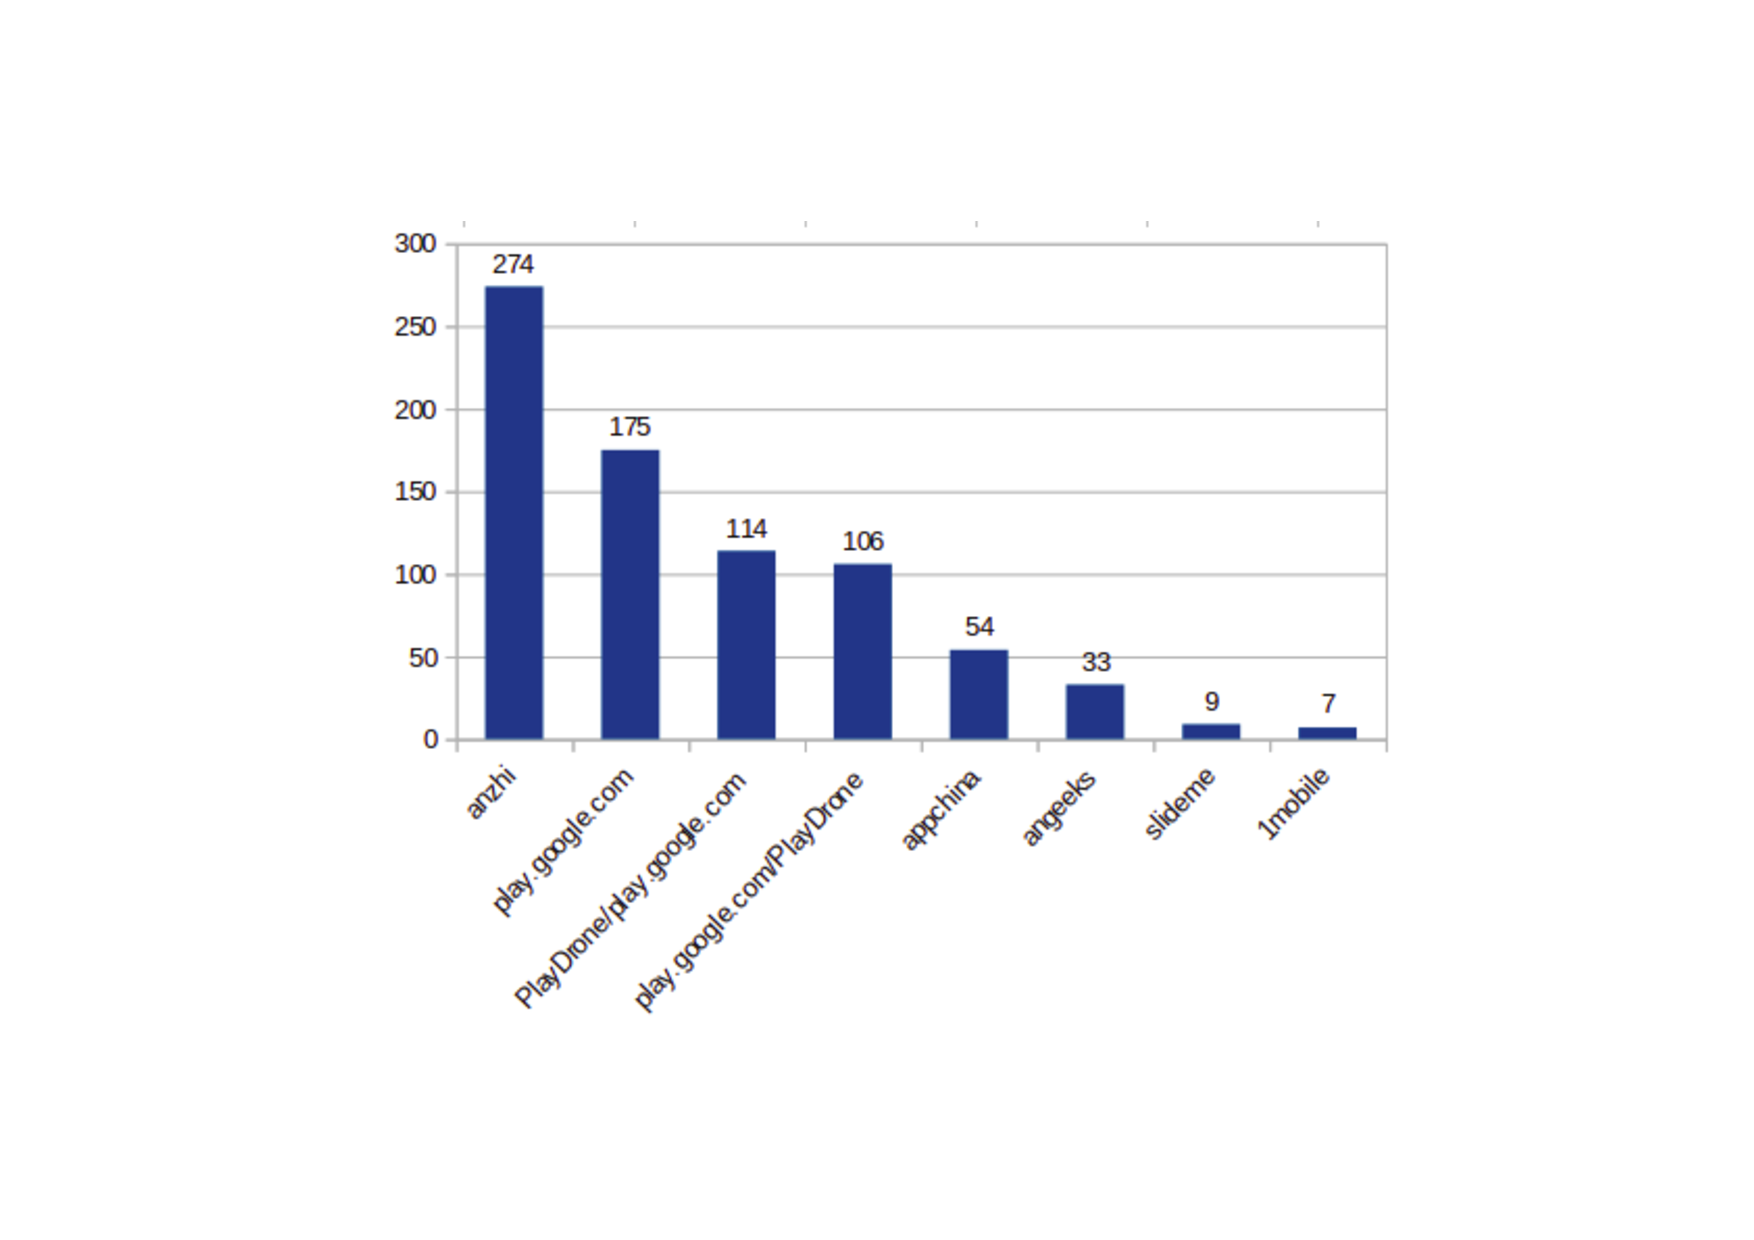
\includegraphics[scale=0.43]{images/stores.pdf}
\caption{Markets where malware was discovered.}
 \label{fig:stores}
\end{figure}


\subsection{Data Collection Procedures} \label{sec:dataCollectionProc}


We take advantage of the DroidXP infrastructure~\cite{DBLP:conf/scam/CostaMCMVBC20}
for data collection. DroidXP allows researchers to compare 
test case generation tools in terms of malicious app behaviors identification, using the \mas. Although the comparison of test
case generation tools is not the goal of this paper, DroidXP
was still useful for automating the following steps of our study.


\begin{enumerate}[S1]
 \item \textbf{Instrumentation}: In the first step,
we configure DroidXP to instrument all pairs of apps in our dataset.
Here, we instrument both versions of the apps (as APK files) to collect relevant information during their execution. Under the hood, DroidXP leverages
DroidFax~\cite{DBLP:conf/icsm/CaiR17a} to instrument the apps and collect static
information about them. To improve the performance across multiple executions,
this phase executes only once for each version of the apps in our dataset.

\item \textbf{Execution}: In this step, DroidXP first installs the (instrumented) version of the APK files in the Android emulator we use in our experiment (API 28) and then starts a test case generation tool for executing both apps version (benign amd malicious). To execute the app, our study builds upon DroidBot~\cite{DBLP:conf/icse/LiYGC17}, since previous works report the best accuracy of the sandboxes built using the \mas and the DroidBot as test case generation tool. To also ensure that each execution gets the benefit of running on a fresh Android instance without biases that could stem out of history, DroidXP wipes out all data stored on the emulator that has been collected from previous executions.


\item \textbf{Data Collection}: During the execution of the instrumented app, we collect all relevant information (such as calls to sensitive APIs, test coverage metrics, and so on). We use this information to analyse the performance of the \mas for detecting malicious behavior. In this paper we extended DroidXP with a new component (DroidXPTrace), which allows us to investigate dynamic call graphs from the outcomes of a DroidXP execution. This was not possible using the vanilla version of DroidXP.
\end{enumerate}

\subsection{Data Analysis Procedures} \label{sec:dataAnalysisProc}

We use basic statistics (average) to identify the
accuracy of the \mas to identify malware, in both
datasets we use in our research---i.e., the original
one with 102 pairs of apps and our curated dataset with
1204 pairs. We use the Spearman Correlation~\cite{spearman-correlation} method and
Logistic Regression~\cite{statistical-learning} to understand the strengths of
the associations between the similarity index, the type and family of a
malware with the mining sandbox approach accuracy---that is,
if the approach was able or not to identify the malicious behavior.
To this particular goal, we consider
both the vanilla implementation and our extended implementation
of the \mas that executes the trace assessment, which allow us
to answer our third research question. 


\subsection{Environment Configuration}\label{sec:hardware}

\todo[inline]{RB: later, if we need space, we can safely comment this section out.}

We deployed our experiment on a 32-Core, AMD EPYC 7542 CPU, 512 GB RAM, storage Samsung SSD 970 EVO 1TB machine running a 64-bit Debian  GNU/Linux 11. We also configured our emulator to run all selected apps on Google Android version 9.0, API 28, 512M SD Card, 7GB internal storage, with X86 ABI image.
For our study, we configured DroidXP to run each of the 1204 app pairs using DroidBot for 3 minutes. To mitigate noise, we repeated the full process 3 times,  which took around 421 machine hours in total. Although it was possible to run more than 10 emulators in parallel on one physical machine, to avoid any interference resulting from context switching within the operating system, we chose to run one emulator at a time. \rb{I don't know if the following is relevant\ldots} Hence, all processes took around 22 days, 17 days for experiment execution and additional 5 days for environment configuration.

